%------------------------------------------------------------------------
% Chapter:  RMC simulation
%------------------------------------------------------------------------

\chapter{Reverse Monte Carlo \label{rmc}}

This chapter gives a short introduction into the RMC level of 
\discus. \Discus can be used to either refine the scattering
intensities directly of to refine the atomic pair distribution
function (PDF) (see chapter \ref{pdf}). A more detailed description of the
various commands can be found in the reference manual or the online
help function.

%------------------------------------------------------------------------

\section{Introduction \label{rmc-int}}

The {\bf R}everse {\bf M}onte {\bf C}arlo (RMC) method
\citep{mcpu88} is another application of the Monte Carlo algorithm
discussed in chapter \ref{mc}.  Here, rather than minimizing the
total energy of the crystal, the difference between observed and
calculated intensity is minimized. Although the method has been
around for about 10 years, the method was first applied to {\it
single crystal} diffuse scattering in a neutron diffraction study on
ice {\it Ih} \citep{nikemc95}. \par

The RMC process starts also with the selection of a random site
and changing its variables like occupancy or displacement by a
random amount. The scattering intensity is recalculated for the
generated move and the goodness-of-fit parameter $\chi^{2}$ as
given in equation \ref{eq-chi2-1} is computed.
%
\begin{equation}
    \chi^{2} = \sum_{i=1}^{N} \frac { [ I_{e}({\bf h}_{i}) -
               I_{c}({\bf h}_{i}) ] ^{2}} { \sigma^{2} }
    \label{eq-chi2-1}
\end{equation}
%
The sum is over all measured data points ${\bf h}_{i}$, $I_{e}$
stands for the experimental and $I_{c}$ for the calculated
intensity.  The change in the goodness-of-fit is given by $\Delta
\chi^{2} = \chi_{old}^{2} - \chi_{new}^{2}$.  Every move which
improves the fit to the data ($\Delta \chi^{2} < 0$) is accepted.
Those moves which worsen the fit ($\Delta \chi^{2} > 0$) are
accepted with a probability of $P = exp(-\Delta \chi^{2} / 2)$. The
parameter $\sigma$ is assumed to be independent of {\bf h} and is
treated as a parameter of the modeling.  The value $\sigma$ can be
identified with the temperature T in the (direct) Monte Carlo method
described in chapter \ref{mc}.  How many {\it bad} moves are
accepted depends on the value of $\sigma$ or T.  \par

%------------------------------------------------------------------------

\section{RMC in more detail \label{rmc-detail}}

For practical use it is necessary to include a scaling factor $f$
and a background parameter $b$ in the definition of the
goodness-of-fit $\chi^{2}$. A weight $w({\bf h})$ is included as
well. \Discus allows the user to choose a particular weighting
scheme or to read weights from a separate input file. The definition
of $\chi^{2}$ used in the program is given in equation
\ref{eq-chi2-2}.
%
\begin{equation}
    \chi^{2} = \sum_{i=1}^{N} \frac { w({\bf h}_{i}) [ I_{e}({\bf h}_{i}) -
               (f \cdot I_{c}({\bf h}_{i}) + b) ] ^{2}} { \sigma^{2} }
    \label{eq-chi2-2}
\end{equation}
%
As in the previous section $I_{e}({\bf h}_{i})$ stands for the
measured intensity at the reciprocal point ${\bf h}_{i}$, and
$I_{c}({\bf h}_{i})$ is the calculated intensity in that point. The
summation is over all N experimental data points.  The value
$\sigma$ is a parameter of the modeling and controls the fraction of
{\it bad} moves which are accepted. The corresponding parameter in
(direct) Monte Carlo simulations is the temperature T.\par

Three different ways to calculate the scale $f$ and background $b$
are implemented. First the user can define fixed values for both:
$f = f_{0}, b = b_{0}$. Secondly, the background can be set to a
fixed value $b = b_{0}$ and the scaling factor $f$ is computed
according to equation \ref{eq-fb0}.
%
\begin{equation}
    f = \frac {\sum\limits_{i=1}^{N} w({\bf h}_{i}) I_{e}({\bf h}_{i})
                                             I_{c}({\bf h}_{i})
       - b_{0} \sum\limits_{i=1}^{N} w({\bf h}_{i}) I_{c}({\bf h}_{i})}
              {\sum\limits_{i=1}^{N} w({\bf h}_{i}) I_{c}^{2}({\bf h}_{i}) }
    \label{eq-fb0}
\end{equation}
%
Alternatively both values $f$ and $b$ can be refined during the
RMC refinement. Equation \ref{eq-fb} shows the corresponding
definitions.
%
\begin{eqnarray}
    f & = & \frac{\sum\limits_{i=1}^{N} w({\bf h}_{i})
                  \sum\limits_{i=1}^{N} w({\bf h}_{i})
                                        I_{e}({\bf h}_{i})I_{c}({\bf h}_{i})
                - \sum\limits_{i=1}^{N} w({\bf h}_{i}) I_{e}({\bf h}_{i})
                  \sum\limits_{i=1}^{N} w({\bf h}_{i}) I_{c}({\bf h}_{i})}
               {  \sum\limits_{i=1}^{N} w({\bf h}_{i})
                  \sum\limits_{i=1}^{N} w({\bf h}_{i}) I_{c}^{2}({\bf h}_{i})
         - \left (\sum\limits_{i=1}^{N} w({\bf h}_{i})
                                        I_{c}({\bf h}_{i}) \right ) ^{2} }
    \nonumber  \\
    b & = & \frac{\sum\limits_{i=1}^{N} w({\bf h}_{i}) I_{e}({\bf h}_{i})
        - f \cdot \sum\limits_{i=1}^{N} w({\bf h}_{i}) I_{c}({\bf h}_{i})}
                 {\sum\limits_{i=1}^{N} w({\bf h}_{i})}
    \label{eq-fb}
\end{eqnarray}
%
The scaling factor which the program prints on the screen during the
RMC refinement is actually (for some yet unknown reason) $1/f$.  The
parameters f and b are computed during each RMC cycle and usually
have large starting values as long as there are big differences
between calculated and observed data.  After every RMC move the
resulting scattering intensity and the $\chi^{2}$ value is
calculated.  In order to save computing time only the contribution
of the modified atoms to the scattering is calculated.  The
difference $\Delta \chi^{2} = \chi_{old}^{2} - \chi_{new}^{2}$ is
taken to decide if the move will be accepted or not.  If $\Delta
\chi^{2} < 0$ the agreement between calculated and measured data has
improved and the move is accepted.  Moves which result in a $\Delta
\chi^{2} > 0$ are only accepted with a probability of $P =
exp(-\Delta \chi^{2} / 2)$.  As the value of $\Delta \chi^{2}$ is
proportional to $1 / \sigma^{2}$, the value of $\sigma$ has an
influence on the amount of {\it bad} moves which will be accepted.
Obviously there are two extremes: For very large values of $\sigma$,
the experimental data are ignored ($\chi^{2} \approx 0$) and with
very small values of $\sigma$ the fit ends up in the local minimum
closest to the starting point, because there is a negligible
probability for {\it bad} moves.  In order to be more independent of
the actual number of data points used, the goodness-of-fit parameter
used in the program is given by $\chi^{2} / \sum w({\bf h}_{i})$.
The program calculates separate scaling factors and background
parameters for every used plane of experimental data.  This allows
to simultaneously use data measured with X-rays and neutrons,
different wavelengths or from different instruments.  The
goodness-of-fit $\chi^{2}$ is displayed as its total value and
separate for each data plane.

%------------------------------------------------------------------------

\section{Setting up a model crystal \label{rmc-cryst}}

The first step in an RMC refinement is the creation of a model
crystal of suitable size.  In many cases the starting structure will
be the (known) average structure for the compound under
investigation.  Since certain information of the crystal (e.g.
symmetry) is used in the RMC segment, it is advisable to {\bf to set
the crystal before entering the RMC segment}. Depending on the kind
of disorder to be modeled it might be necessary to introduce
displacements according to the temperature factors (command 'therm',
see section \ref{mod-therm}) or create the needed amount of
vacancies before starting the RMC refinement.  How to generate a
crystal is described in chapter \ref{struc}, tools to modify the
crystal are discussed in chapters \ref{mod-simple} and
\ref{mod}.\par

%------------------------------------------------------------------------

\section{Operation modes \label{rmc-mode}}

So far changes to the crystal made during the RMC refinement were
simply called 'moves'. These moves can either be a displacement of
an atom or the change of the occupancy of an atom site.  Because the
relative abundance of the elements is not allowed to change during
the simulation, the later move is actually made by switching the
atoms of two sites within the crystal. The program knows three
different operation modes which involve three different kinds of
moves shown in figure \ref{rmc-fig1}. Additionally user defined
moves can be included in an external subroutine linked to the
program \discus.
%
\begin{figure}[!tbh]
   \centering
   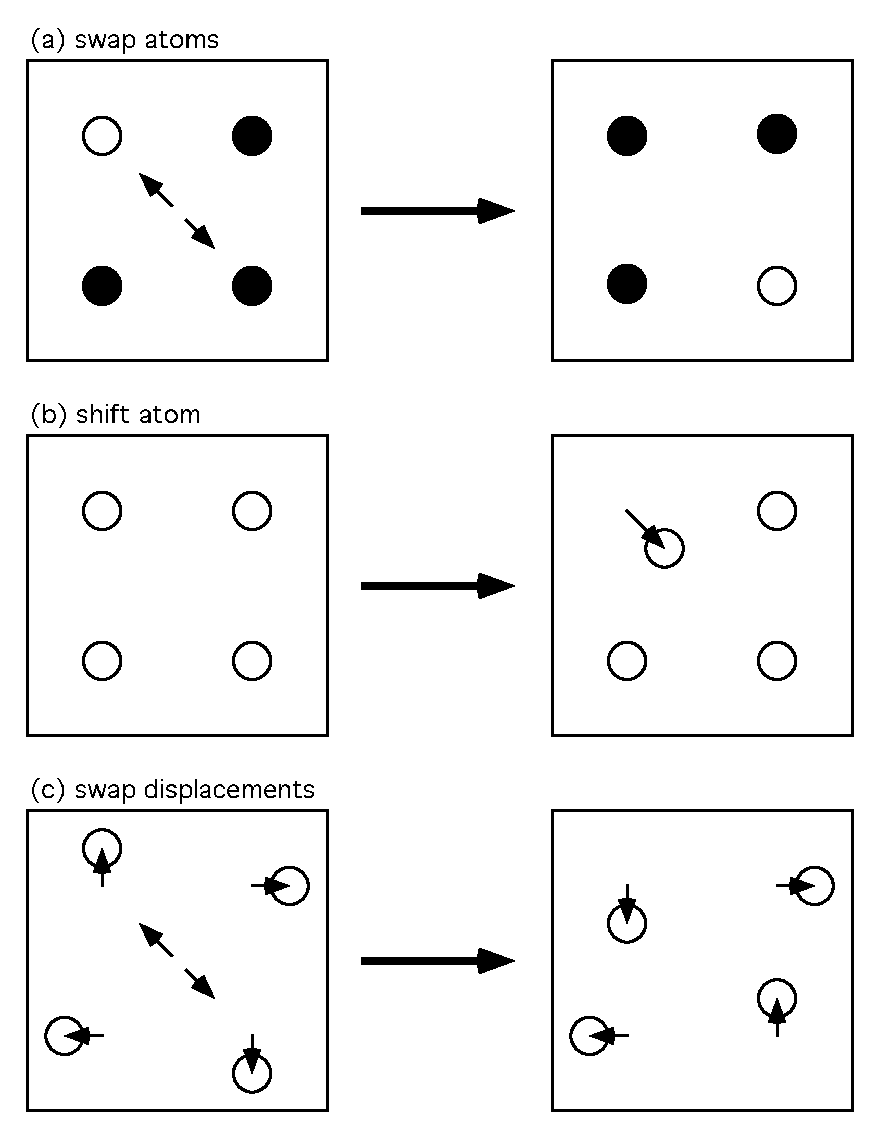
\includegraphics[scale=0.5, angle=0]{rmc.1.eps}
   \caption{RMC operation modes of \Discus }
   \label{rmc-fig1}
\end{figure}
%
A short description of the different RMC operation modes is given in
the list below.
%
\begin{enumerate}
    \item {\it switch chemistry}:
    This mode (Fig. \ref{rmc-fig1}a) allows to simulate occupational disorder
    by selecting two different atoms randomly and switch these two atoms. This
    operation mode can obviously work only, if at least two different types of
    atoms are present within the crystal.  This mode is selected by the
    command {\tt set mode, swchem}.

    \item {\it shift atom}:
    If this mode (Fig.  \ref{rmc-fig1}b) is set, a randomly selected atom is
    shifted by a random amount in a random direction.  The size of the
    generated shift is chosen uniformly in the interval [-1,1] unit cell.
    The actual shift applied to the atom is the generated shift multiplied
    with a user defined factor ('set move,$<$x$>$,$<$y$>$,$<$z$>$').
    These factors are also given in unit cell units.  The shift mode is
    selected by with {\tt set mode, shift}.

    \item {\it switch displacements}:
    This mode (Fig. \ref{rmc-fig1}c) is selected by the command {\tt set
    mode, swdisp} by swapping the displacement, i.e.  the difference between
    the average and the actual position, of two randomly selected atoms of
    the same type and thus the overall average displacements remain constant
    in contrast the previous mode.  The user has to make sure that initial
    displacements are present in the starting structure (e.g.  thermal
    displacements e.g.  by using the command {\tt therm}.

    \item {\it external}:
    The program \Discus allows the user to define more complex RMC
    moves via an external subroutine.  This subroutine is defined in the file
    {\it extrmc.f90}. For more details about the construction of such a
    subroutine, read the commented example in the file {\it extrmc.f90}
    which is part of the distribution.
\end{enumerate}
%
The program allows to select ({\tt sele $<$typ1$>$, $<$typ2$>$, ..})
and deselect ({\tt dsel $<$typ1$>$, $<$typ2$>$, ..}) atom types
which should be taken into account during the RMC simulation.
Alternatively molecules (if present) can be selected using the
commands {\tt msel $<$typ1$>$, $<$typ2$>$,..} and {\tt mdes
$<$typ1$>$, $<$typ2$>$, ..}. Here $<$typ$>$ is the corresponding
molecule type. All modes listed above can be used for these rigid
molecules as well.  Rotations and other symmetry operations can be
realized by creating the wanted different orientations of the
molecules as different types using the symmetry segment of 
\Discus (see chapter \ref{cryst-sym}) and subsequently using the
'swap chemistry' mode. After every generated move the minimal
allowed distances ({\tt set mdis, $<$atom1$>$, $<$atom1$>$,
$<$dist$>$}) between all selected atoms are checked and if atoms are
too close, the move is rejected.

%------------------------------------------------------------------------

\section{Running RMC \label{rmc-run}}

Finally, the experimental data need to be read before the RMC
refinement can start.  The file format for the experimental input
data is similar to the output formats \Kuplot and {\it PGM} for
the Fourier transform.  It might be necessary to remove Bragg peaks
and other unwanted scattering (e.g.  powder rings from a sample
holder) from the input data set. With the {\tt data} command, the
method (neutron or X-ray), weighting scheme and the corners of the
input data set in reciprocal space are entered.  More than one plane
of experimental data can be read by repeating the 'data' command.
After the data have been read, select the desired RMC mode, select
the appropriate atoms and start the refinement with the {\tt run}
command.
%

\begin{MacVerbatim}
   Gen:   1200 try:    352 acc: (good/bad):     62 /      0 s2x2:   11829643.
     Plane  1: scal:  14.83     / back:  22.23     / s2x2:          11829643.
\end{MacVerbatim}
%
The screen output is updated in a user defined interval, an example
output is shown above.  The fist line gives the number of generated
moves ('Gen') and how many of those were actually tested ('try').
The difference is due to selecting atoms that should not take part
in the refinement and moves that violate minimal atom distances. The
next two numbers give the number of good ($\Delta \chi^{2} < 0$) and
bad ($\Delta \chi^{2} > 0$) moves that have been accepted.  The last
number is the current value of the overall $\chi^{2}$ for all data
planes.  Additionally the scaling factor $f$ and the background $b$
are given for each data plane (one in this example) followed by
$\chi^{2}$ for the corresponding data plane.  The resulting
structure as well as the calculated scattering can be saved with the
{\tt save} command.

%------------------------------------------------------------------------
